\documentclass[aspectratio=169,11pt]{ctexbeamer}

\usetheme{Madrid}
\usecolortheme{default}
\setbeamertemplate{navigation symbols}{}

\usepackage{amsmath,amssymb,mathtools,bm}
\usepackage{graphicx}
\usepackage{tikz}
\usepackage{pgfplots}
\usepackage{array}
\usepackage{booktabs}
\usepackage{multicol}
\usetikzlibrary{arrows.meta,calc,intersections,decorations.pathreplacing}
\pgfplotsset{compat=1.18}

\newcommand{\R}{\mathbb{R}}
\newcommand{\osc}{\omega}



% Unified Yingxing Beamer footer and visual style.
\newcommand{\huayinglogo}{assets/logo1.jpg}
\newcommand{\huayingslogan}{英行培优，成绩无忧；英行相伴，刮目相看}

\setbeamersize{text margin left=8mm,text margin right=8mm}
\setbeamerfont{frametitle}{size=\large}
\setbeamercolor{structure}{fg=blue!70!black}
\setbeamercolor{frametitle}{bg=blue!75!black,fg=white}
\setbeamercolor{block title}{bg=blue!10,fg=black}
\setbeamercolor{block body}{bg=blue!2,fg=black}
\setbeamercolor{author in head/foot}{bg=blue!8,fg=black}
\setbeamercolor{title in head/foot}{bg=blue!8,fg=black}

\setbeamertemplate{footline}{%
  \leavevmode%
  \hbox{%
    \begin{beamercolorbox}[wd=.12\paperwidth,ht=3.8ex,dp=1.2ex,center]{author in head/foot}%
      \includegraphics[height=2.9ex]{\huayinglogo}%
    \end{beamercolorbox}%
    \begin{beamercolorbox}[wd=.76\paperwidth,ht=3.8ex,dp=1.2ex,center]{title in head/foot}%
      \scriptsize \huayingslogan
    \end{beamercolorbox}%
    \begin{beamercolorbox}[wd=.12\paperwidth,ht=3.8ex,dp=1.2ex,right]{author in head/foot}%
      \scriptsize \insertframenumber/\inserttotalframenumber\hspace*{1em}
    \end{beamercolorbox}%
  }%
}

\title{闭区间上连续函数的性质}
\subtitle{最值定理、零点定理、一致连续与振幅}
\author{王晨旭}
\date{}

\begin{document}

\begin{frame}
  \titlepage
\end{frame}

\begin{frame}{本讲主线}
\begin{itemize}
  \item 闭区间上的连续函数比一般区间上的连续函数更“规整”。
  \item 三条主线：
  \begin{enumerate}
    \item 有界与取到最值；
    \item 零点、介值与值域为区间；
    \item 一致连续以及振幅刻画。
  \end{enumerate}
  \item 核心方法反复出现：
  \[
    \text{局部连续性}+\text{闭区间紧性}\Longrightarrow \text{整体结论}.
  \]
\end{itemize}
\end{frame}

\begin{frame}{定理 1：有界性定理}
\textbf{结论：}若 $f(x)$ 在闭区间 $[a,b]$ 上连续，则 $f$ 在 $[a,b]$ 上有界。
\[
  f\in C[a,b]\Longrightarrow \exists M>0,\ \forall x\in[a,b],\ |f(x)|\le M.
\]
\vspace{0.5em}
\textbf{提醒：}
\begin{itemize}
  \item “连续”给的是局部控制；
  \item “闭区间”把局部控制提升成整体控制；
  \item 若去掉闭区间条件，结论可能失效。
\end{itemize}
\[
  f(x)=\frac1x \text{ 在 }(0,1]\text{ 上连续，但无界。}
\]
\end{frame}

\begin{frame}{有界性定理：证法一}
\textbf{反证法。} 假设 $f$ 在 $[a,b]$ 上无界，则存在点列 $\{x_n\}\subset[a,b]$，使得
\[
  |f(x_n)|\ge n,\qquad n=1,2,\cdots
\]
由于 $\{x_n\}$ 是有界点列，存在收敛子列 $\{x_{n_i}\}$，满足
\[
  x_{n_i}\to x_0\in[a,b].
\]
又因为 $f$ 在 $x_0$ 处连续，
\[
  f(x_{n_i})\to f(x_0).
\]
这说明 $\{f(x_{n_i})\}$ 有界，但这与
\[
  |f(x_{n_i})|\ge n_i\to+\infty
\]
矛盾，从而 $f$ 必有界。
\end{frame}

\begin{frame}{有界性定理：证法二}
对每个 $x\in[a,b]$，由连续性存在 $\delta_x>0$，使得
\[
  |f(x')-f(x)|\le 1,\qquad \forall x'\in(x-\delta_x,x+\delta_x)\cap[a,b].
\]
于是开区间族
\[
  \bigl\{(x-\delta_x,x+\delta_x)\cap[a,b]\bigr\}_{x\in[a,b]}
\]
构成 $[a,b]$ 的一个开覆盖。由闭区间的紧性，可取有限子覆盖
\[
  (x_i-\delta_{x_i},x_i+\delta_{x_i})\cap[a,b],\qquad i=1,2,\dots,k.
\]
令
\[
  M=\max_{1\le i\le k}\bigl(|f(x_i)|+1\bigr),
\]
则任意 $x\in[a,b]$ 必属于某个子覆盖区间，从而 $|f(x)|\le M$。
\end{frame}

\begin{frame}{定理 2：最值定理}
\textbf{结论：}若 $f$ 在闭区间 $[a,b]$ 上连续，则 $f$ 在 $[a,b]$ 上能取到最大值和最小值。
\[
  \exists x_*,x^*\in[a,b],\quad f(x_*)\le f(x)\le f(x^*),\ \forall x\in[a,b].
\]
\vspace{0.6em}
\textbf{关键区别：}
\begin{itemize}
  \item 有界性只保证 $\sup f([a,b])$、$\inf f([a,b])$ 存在；
  \item 最值定理进一步保证这两个界确实被函数取到。
\end{itemize}
\end{frame}

\begin{frame}{最值定理：证明思路}
由有界性定理，$M=\sup f([a,b])$ 存在。按上确界定义，可取 $\{x_n\}\subset[a,b]$ 使
\[
  M-\frac1n\le f(x_n)\le M.
\]
由于 $\{x_n\}$ 有界，存在收敛子列 $x_{n_i}\to x^*\in[a,b]$。由连续性得
\[
  f(x_{n_i})\to f(x^*).
\]
而同时 $f(x_{n_i})\to M$，故
\[
  f(x^*)=M.
\]
因此最大值被取到。最小值同理，或对 $-f$ 使用最大值定理。
\end{frame}

\begin{frame}{闭区间条件不可削弱}
\begin{columns}[T]
\column{0.52\textwidth}
\textbf{最值定理失效例：}
\[
  f(x)=x,\qquad x\in(0,1].
\]
\begin{itemize}
  \item 在 $(0,1]$ 上连续；
  \item 有最大值 $1$；
  \item 但没有最小值。
\end{itemize}

\column{0.44\textwidth}
\begin{tikzpicture}[scale=0.92]
  \draw[->] (-0.1,0)--(3.2,0) node[right] {$x$};
  \draw[->] (0,-0.1)--(0,3.0) node[above] {$y$};
  \draw[thick,domain=0.35:3,smooth] plot(\x,\x);
  \filldraw[white] (0.35,0.35) circle(2.2pt);
  \fill (3,3) circle(2pt);
  \draw[dashed] (3,0)--(3,3);
  \draw[dashed] (0,3)--(3,3);
  \node[below] at (0.35,0) {$0$};
  \node[below] at (3,0) {$1$};
  \node[left] at (0,3) {$1$};
\end{tikzpicture}
\end{columns}
\vspace{0.4em}
连续函数在开区间上可以“逼近”某个界，但不一定“取到”它。
\end{frame}

\begin{frame}[allowframebreaks]{定理 3：零点定理}
若 $f$ 在 $[a,b]$ 上连续，且
\[
  f(a)f(b)<0,
\]
则存在 $\xi\in(a,b)$，使得
\[
  f(\xi)=0.
\]
\begin{center}
\begin{tikzpicture}[scale=0.95]
  \draw[->] (-3.3,0)--(3.7,0) node[right] {$x$};
  \draw[->] (0,-2.2)--(0,2.7) node[above] {$y$};
  \draw[thick,domain=-3:3.2,samples=200,smooth]
    plot(\x,{0.08*(\x+2.6)*(\x-1.2)*(\x-2.2)+0.35});
  \draw[dashed] (-2.6,0)--(-2.6,-0.65);
  \draw[dashed] (3.0,0)--(3.0,1.15);
  \draw[dashed] (0,-0.65)--(-2.6,-0.65);
  \draw[dashed] (0,1.15)--(3.0,1.15);
  \node[below] at (-2.6,0) {$a$};
  \node[below] at (3.0,0) {$b$};
  \node[below] at (1.55,0) {$\xi$};
  \node[left] at (0,-0.65) {$f(a)$};
  \node[left] at (0,1.15) {$f(b)$};
\end{tikzpicture}
\end{center}
\end{frame}

\begin{frame}[allowframebreaks]{零点定理：区间套证明}
不妨设
\[
  f(a)<0<f(b).
\]
将 $[a,b]$ 二等分，取中点 $m_1=\dfrac{a+b}{2}$。若 $f(m_1)=0$，结论成立；否则在两半区间中必有一半仍满足两端异号，记为 $[a_1,b_1]$。

继续二分，得到闭区间套
\[
  [a_1,b_1]\supset[a_2,b_2]\supset\cdots\supset[a_n,b_n]\supset\cdots
\]
且
\[
  f(a_n)\le 0,\qquad f(b_n)\ge 0,\qquad b_n-a_n=\frac{b-a}{2^n}\to 0.
\]
由闭区间套定理，存在 $x_0\in[a,b]$ 使
\[
  a_n\to x_0,\qquad b_n\to x_0.
\]
再由连续性，
\[
  0\ge \lim_{n\to\infty}f(a_n)=f(x_0)=\lim_{n\to\infty}f(b_n)\ge 0,
\]
故 $f(x_0)=0$。
\end{frame}

\begin{frame}{零点定理：上确界证明}
令
\[
  A=\{x\in[a,b]\mid f(x)<0\}.
\]
则 $a\in A$，而且 $A$ 有上界，因此 $\xi=\sup A$ 存在。
\vspace{0.5em}

由连续性证明：
\begin{itemize}
  \item 不能有 $f(\xi)<0$，否则 $\xi$ 右侧还有点属于 $A$，与上确界矛盾；
  \item 也不能有 $f(\xi)>0$，否则 $\xi$ 左侧附近都满足 $f>0$，这与 $\xi$ 是 $A$ 的上确界矛盾。
\end{itemize}
因此只能是
\[
  f(\xi)=0.
\]
\vspace{0.5em}
\textbf{要点：} 连续性保证了符号不能“突然跳变”。
\end{frame}

\begin{frame}{定理 4：介值定理}
设 $f$ 在 $[a,b]$ 上连续，$\mu$ 是严格介于 $f(a)$ 和 $f(b)$ 之间的数，则存在 $\xi\in(a,b)$ 使
\[
  f(\xi)=\mu.
\]
\vspace{0.5em}
\textbf{证明：} 考虑函数
\[
  F(x)=f(x)-\mu.
\]
因为 $F$ 仍连续，且
\[
  F(a)F(b)=\bigl(f(a)-\mu\bigr)\bigl(f(b)-\mu\bigr)<0,
\]
由零点定理，存在 $\xi\in(a,b)$ 使
\[
  F(\xi)=0,
\]
即
\[
  f(\xi)=\mu.
\]
\end{frame}

\begin{frame}{推论：连续函数的像仍为区间}
若 $f$ 在闭区间 $[a,b]$ 上连续，设
\[
  m=\min_{x\in[a,b]}f(x),\qquad M=\max_{x\in[a,b]}f(x),
\]
则
\[
  f([a,b])=[m,M].
\]
\vspace{0.5em}
\textbf{理由：}
\begin{itemize}
  \item 由最值定理，$m,M$ 被取到；
  \item 由介值定理，$m$ 与 $M$ 之间的每一个值都被取到。
\end{itemize}
\vspace{0.5em}
更一般地，若 $I$ 是区间，$f$ 在 $I$ 上连续，则 $f(I)$ 仍是区间。
\end{frame}

\begin{frame}{推论 2：可逆与严格单调}
设 $f$ 是区间 $I$ 上的连续函数，则
\[
  f \text{ 可逆}\Longleftrightarrow f \text{ 在 }I\text{ 上严格单调}.
\]
\begin{columns}[T]
\column{0.48\textwidth}
\textbf{为什么严格单调足够？}
\begin{itemize}
  \item 严格单调 $\Rightarrow$ 单射；
  \item 连续 $\Rightarrow$ 值域为区间；
  \item 因此反函数在值域上有良好定义。
\end{itemize}

\column{0.48\textwidth}
\textbf{为什么可逆必严格单调？}
\begin{itemize}
  \item 若不严格单调；
  \item 借助介值定理会出现同一函数值对应多个点；
  \item 这与可逆矛盾。
\end{itemize}
\end{columns}
\end{frame}

\begin{frame}{一个应用：不动点存在定理}
若
\[
  f:[a,b]\to[a,b]
\]
连续，则存在 $\xi\in[a,b]$ 使得
\[
  f(\xi)=\xi.
\]
\vspace{0.5em}
\textbf{证明：} 令
\[
  F(x)=f(x)-x.
\]
由于 $f(a)\in[a,b]$，故 $F(a)=f(a)-a\ge 0$；同理 $F(b)=f(b)-b\le 0$。于是
\[
  F(a)F(b)\le 0.
\]
由零点定理及其注记，存在 $\xi\in[a,b]$，使
\[
  F(\xi)=0,
\]
即 $f(\xi)=\xi$。
\end{frame}

\begin{frame}{又一个应用：奇数次多项式必有实根}
设
\[
  P(x)=a_0x^{2n-1}+a_1x^{2n-2}+\cdots+a_{2n-1},\qquad a_0\ne 0.
\]
则 $P(x)$ 至少有一个实根。
\vspace{0.5em}

\textbf{理由：}
\begin{itemize}
  \item 多项式在 $\R$ 上连续；
  \item 当 $x\to+\infty$ 与 $x\to-\infty$ 时，奇数次首项决定两端符号相反；
  \item 因此存在 $x_1<x_2$ 使 $P(x_1)P(x_2)<0$；
  \item 再由零点定理，存在 $\xi\in(x_1,x_2)$ 使 $P(\xi)=0$。
\end{itemize}
\end{frame}

\begin{frame}{定义 1：一致连续}
设函数 $f$ 定义在区间 $I$ 上。若任给 $\varepsilon>0$，均存在
\[
  \delta=\delta(\varepsilon)>0,
\]
使得当 $x_1,x_2\in I$ 且 $|x_1-x_2|<\delta$ 时，有
\[
  |f(x_1)-f(x_2)|<\varepsilon,
\]
则称 $f$ 在 $I$ 上\textbf{一致连续}。
\vspace{0.5em}

\textbf{与普通连续的区别：}
\[
  \text{连续： }\delta=\delta(\varepsilon,x_0),\qquad
  \text{一致连续： }\delta=\delta(\varepsilon).
\]
\end{frame}

\begin{frame}{连续与一致连续的差别}
\begin{columns}[T]
\column{0.5\textwidth}
\textbf{普通连续}
\begin{itemize}
  \item 针对某个固定点 $x_0$；
  \item 允许 $\delta$ 依赖于 $x_0$；
  \item 是局部性质。
\end{itemize}

\column{0.5\textwidth}
\textbf{一致连续}
\begin{itemize}
  \item 面向整个区间 $I$；
  \item 同一个 $\delta$ 适用于所有点；
  \item 是整体性质。
\end{itemize}
\end{columns}
\vspace{0.7em}
因此：
\[
  \text{一致连续}\Longrightarrow \text{连续},
\]
但反过来在一般区间上不成立。
\end{frame}

\begin{frame}{连续但不一致连续：一个标准反例}
考虑函数
\[
  f(x)=x^2,\qquad x\in\R.
\]
\textbf{性质：}
\begin{itemize}
  \item $f$ 在 $\R$ 上处处连续；
  \item 但 $f$ 在 $\R$ 上并不一致连续。
\end{itemize}
\vspace{0.5em}

\textbf{直观原因：}
当 $x$ 很大时，即使两个点相距很小，平方后函数值的差也可能很大。
\[
  (x+h)^2-x^2=2xh+h^2.
\]
其中 $2xh$ 会随着 $x$ 的增大而变大，所以不存在对整个 $\R$ 都适用的统一 $\delta$。
\end{frame}

\begin{frame}[allowframebreaks]{反例解答：$x^2$ 在 $\R$ 上不一致连续}
若 $x^2$ 在 $\R$ 上一致连续，则对 $\varepsilon=1$，存在 $\delta>0$，使得
\[
  |x-y|<\delta \Longrightarrow |x^2-y^2|<1,\qquad \forall x,y\in\R.
\]
取
\[
  x_n=n,\qquad y_n=n+\frac{1}{n}\qquad (n\ge 1).
\]
则
\[
  |x_n-y_n|=\frac1n\to 0.
\]
但
\begin{align*}
  |x_n^2-y_n^2|
  &=\left|n^2-\left(n+\frac1n\right)^2\right| \\
  &=\left|2+\frac1{n^2}\right|
  >1.
\end{align*}
这与一致连续矛盾，因此 $f(x)=x^2$ 在 $\R$ 上连续，但不一致连续。
\end{frame}

\begin{frame}{例题 1}
研究函数
\[
  f(x)=\sin\dfrac1x,\qquad x\in(0,+\infty)
\]
的一致连续性。
\end{frame}

\begin{frame}{例题 1：解答}
取
\[
  a_n=\frac{1}{2n\pi},\qquad b_n=\frac{1}{2n\pi+\frac{\pi}{2}},\qquad n\ge 1.
\]
则
\[
  a_n-b_n=\frac{1}{2\pi n(4n+1)}\to 0,
\]
而
\[
  \left|\sin\frac1{a_n}-\sin\frac1{b_n}\right|
  =
  |\sin(2n\pi)-\sin(2n\pi+\tfrac{\pi}{2})|
  =1.
\]
这说明任取多小的 $\delta$，都能找到两点间距小于 $\delta$，但函数值差不小于 $1$。
\vspace{0.4em}

所以 $\sin\dfrac1x$ 在 $(0,+\infty)$ 上\textbf{不是}一致连续的。
\end{frame}

\begin{frame}{例题 2}
研究函数
\[
  f(x)=\sin x,\qquad x\in\R
\]
的一致连续性。
\end{frame}

\begin{frame}{例题 2：解答}
任给 $\varepsilon>0$，令 $\delta=\varepsilon$。当 $|x_1-x_2|<\delta$ 时，
\begin{align*}
  |\sin x_1-\sin x_2|
  &=2\left|\sin\frac{x_1-x_2}{2}\cos\frac{x_1+x_2}{2}\right|\\
  &\le 2\left|\sin\frac{x_1-x_2}{2}\right|\\
  &\le |x_1-x_2|<\varepsilon.
\end{align*}
因此 $\sin x$ 在 $(-\infty,+\infty)$ 上一致连续。
\vspace{0.5em}

更强一点说，
\[
  |\sin x_1-\sin x_2|\le |x_1-x_2|,
\]
因此 $\sin x$ 是一个 Lipschitz 函数。
\end{frame}

\begin{frame}{例题 3}
设函数 $f(x)$ 定义在区间 $I$ 中。若存在常数 $M>0$ 与 $0<\alpha\le 1$，使
\[
  |f(x_1)-f(x_2)|\le M|x_1-x_2|^\alpha,\qquad \forall x_1,x_2\in I,
\]
证明：$f$ 在 $I$ 上一致连续。
\end{frame}

\begin{frame}{例题 3：解答}
若存在常数 $M>0$ 与 $0<\alpha\le 1$，使
\[
  |f(x_1)-f(x_2)|\le M|x_1-x_2|^\alpha,\qquad \forall x_1,x_2\in I,
\]
则称 $f$ 满足 $\alpha$ 阶 H\"older 条件。
\vspace{0.5em}

\textbf{结论：} 任意 H\"older 函数都一致连续。
\vspace{0.5em}

\textbf{证明：} 给定 $\varepsilon>0$，取
\[
  \delta=\left(\frac{\varepsilon}{M}\right)^{1/\alpha},
\]
则当 $|x_1-x_2|<\delta$ 时，
\[
  |f(x_1)-f(x_2)|
  \le M|x_1-x_2|^\alpha
  < M\delta^\alpha
  =\varepsilon.
\]
\end{frame}

\begin{frame}{命题 1：一致连续的封闭性}
若 $f,g$ 在区间 $I$ 上一致连续，则：
\begin{enumerate}
  \item $\alpha f+\beta g$ 在 $I$ 上一致连续；
  \item 若 $f,g$ 有界，则 $fg$ 在 $I$ 上一致连续；
  \item 若 $f$ 有界，且存在 $\varepsilon_0>0$ 使 $g(x)\ge \varepsilon_0$，则 $\dfrac{f}{g}$ 在 $I$ 上一致连续；
  \item 一致连续函数的复合函数仍一致连续。
\end{enumerate}
\vspace{0.5em}
这些结论与普通连续的四则运算、复合运算规律完全平行，只是证明时要处理同一个统一的 $\delta$。
\end{frame}

\begin{frame}{为什么在乘积里要求 $f,g$ 有界？}
要证明 $fg$ 一致连续，常用恒等式
\[
  f(x)g(x)-f(y)g(y)
  =
  f(x)\bigl(g(x)-g(y)\bigr)+g(y)\bigl(f(x)-f(y)\bigr).
\]
于是
\[
  |f(x)g(x)-f(y)g(y)|
  \le |f(x)|\,|g(x)-g(y)|+|g(y)|\,|f(x)-f(y)|.
\]
\vspace{0.5em}

\textbf{关键点：}
\begin{itemize}
  \item 一致连续只能控制 $|f(x)-f(y)|$ 和 $|g(x)-g(y)|$ 很小；
  \item 但前面的系数 $|f(x)|$、$|g(y)|$ 若可能很大，就无法统一压住右边；
  \item 因此通常要先有
  \[
    |f(x)|\le M,\qquad |g(x)|\le N,
  \]
  才能推出
  \[
    |f(x)g(x)-f(y)g(y)|
    \le M|g(x)-g(y)|+N|f(x)-f(y)|.
  \]
\end{itemize}
\end{frame}

\begin{frame}{反例：一致连续函数的乘积未必一致连续}
在 $\R$ 上取
\[
  f(x)=x,\qquad g(x)=x.
\]
\begin{itemize}
  \item $f,g$ 都在 $\R$ 上一致连续；
  \item 但它们都无界。
\end{itemize}
\vspace{0.5em}

此时
\[
  f(x)g(x)=x^2.
\]
而我们已经证明过：
\[
  x^2 \text{ 在 }\R\text{ 上连续，但不一致连续。}
\]
所以“若 $f,g$ 有界，则 $fg$ 一致连续”里的\textbf{有界条件不能随便删掉}。
\end{frame}

\begin{frame}{为什么在商里要求 $f$ 有界且 $g(x)\ge \varepsilon_0>0$？}
考虑
\[
  \frac{f(x)}{g(x)}-\frac{f(y)}{g(y)}
  =
  \frac{f(x)g(y)-f(y)g(x)}{g(x)g(y)}.
\]
把分子拆开：
\[
  f(x)g(y)-f(y)g(x)
  =
  f(x)\bigl(g(y)-g(x)\bigr)+g(x)\bigl(f(x)-f(y)\bigr).
\]
因此
\[
  \left|\frac{f(x)}{g(x)}-\frac{f(y)}{g(y)}\right|
  \le
  \frac{|f(x)|\,|g(y)-g(x)|+|g(x)|\,|f(x)-f(y)|}{|g(x)g(y)|}.
\]
\vspace{0.4em}

\textbf{所以需要两个控制：}
\begin{itemize}
  \item $f$ 有界：控制分子中的 $|f(x)|$；
  \item $g(x)\ge \varepsilon_0>0$：保证分母不接近 $0$，即
  \[
    |g(x)g(y)|\ge \varepsilon_0^2.
  \]
\end{itemize}
\end{frame}

\begin{frame}[allowframebreaks]{商的条件若不满足，会出现什么反例？}
\textbf{反例 1：若 $g$ 不远离 $0$，则结论可能失效。}
\[
  f(x)=1,\qquad g(x)=x,\qquad x\in(0,1].
\]
\begin{itemize}
  \item $f$ 一致连续且有界；
  \item $g$ 在 $(0,1]$ 上一致连续；
  \item 但 $g(x)\not\ge \varepsilon_0>0$，因为 $x\to 0^+$。
\end{itemize}
于是
\[
  \frac{f(x)}{g(x)}=\frac1x,
\]
它在 $(0,1]$ 上\textbf{不是}一致连续。
\vspace{0.7em}

\textbf{反例 2：若 $f$ 不有界，结论也可能失效。}
\[
  f(x)=x,\qquad g(x)=\frac{1}{2+\sin x},\qquad x\in\R.
\]
\begin{itemize}
  \item $f(x)=x$ 在 $\R$ 上一致连续，但无界；
  \item $g$ 在 $\R$ 上一致连续，且
  \[
    \frac13\le g(x)\le 1,
  \]
  因而分母始终远离 $0$。
\end{itemize}
\end{frame}

\begin{frame}[allowframebreaks]{商的反例（二）补全}
对上页的反例 2，
\[
  \frac{f(x)}{g(x)}=x(2+\sin x).
\]
取
\[
  x_n=2n\pi,\qquad y_n=2n\pi+\frac1n.
\]
则
\[
  |x_n-y_n|=\frac1n\to 0.
\]
但
\begin{align*}
  \left|\frac{f(x_n)}{g(x_n)}-\frac{f(y_n)}{g(y_n)}\right|
  &=\left|2x_n-y_n\bigl(2+\sin(y_n)\bigr)\right| \\
  &=\left|4n\pi-\left(2n\pi+\frac1n\right)\left(2+\sin\frac1n\right)\right|.
\end{align*}
由于 $\sin\frac1n\sim \frac1n$，右边趋近于 $2\pi$，特别地不会趋于 $0$。
\vspace{0.5em}

所以 $\dfrac{f}{g}$ 在 $\R$ 上\textbf{不是}一致连续的。  
这说明在商的结论里，$f$ 的有界性也确实不能随便去掉。
\end{frame}

\begin{frame}[allowframebreaks]{更清楚地理解商的条件}
\textbf{结论里写成：}
\[
  f \text{ 有界},\qquad g(x)\ge \varepsilon_0>0
\]
是因为这是最方便、最稳妥的一组充分条件。
\vspace{0.6em}

\textbf{其中：}
\begin{itemize}
  \item $g$ 远离 $0$ 是本质要求，否则 $\dfrac1{g(x)}$ 会在接近零点时爆炸；
  \item $f$ 有界是技术要求，用来保证
  \[
    \frac{f}{g}=f\cdot \frac1g
  \]
  中乘积仍可由“有界 $\times$ 一致连续”来控制。
\end{itemize}
\vspace{0.6em}

\textbf{一个更自然的证明路线：}
\begin{enumerate}
  \item 先由 $g(x)\ge \varepsilon_0>0$ 证明 $\dfrac1g$ 一致连续；
  \item 再由 $f$ 有界且一致连续、$\dfrac1g$ 一致连续，推出
  \[
    \frac{f}{g}=f\cdot \frac1g
  \]
  一致连续。
\end{enumerate}
\end{frame}

\begin{frame}{定理 5：Cantor 定理}
若 $f$ 在闭区间 $[a,b]$ 上连续，则 $f$ 在 $[a,b]$ 上一致连续。
\[
  f\in C[a,b]\Longrightarrow f \text{ 在 }[a,b]\text{ 上一致连续}.
\]
\vspace{0.7em}
\textbf{意义：}
\begin{itemize}
  \item 把逐点连续提升成了整体可控；
  \item 是闭区间上连续函数最重要的全局性质之一；
  \item 后面学习积分、函数列、极限交换时会不断用到。
\end{itemize}
\end{frame}

\begin{frame}{Cantor 定理：反证法证明}
若 $f$ 不是一致连续的，则存在 $\varepsilon_0>0$，以及两列点 $\{a_n\},\{b_n\}\subset[a,b]$，满足
\[
  |a_n-b_n|\to 0,\qquad |f(a_n)-f(b_n)|\ge \varepsilon_0.
\]
由于 $\{b_n\}$ 有界，存在收敛子列 $b_{n_i}\to x_0\in[a,b]$。于是
\[
  a_{n_i}=(a_{n_i}-b_{n_i})+b_{n_i}\to x_0.
\]
由 $f$ 在 $x_0$ 处连续，
\[
  f(a_{n_i})\to f(x_0),\qquad f(b_{n_i})\to f(x_0),
\]
从而
\[
  |f(a_{n_i})-f(b_{n_i})|\to 0,
\]
这与 $|f(a_{n_i})-f(b_{n_i})|\ge \varepsilon_0$ 矛盾。
\end{frame}

\begin{frame}{Cantor 定理：有限覆盖证明}
任给 $\varepsilon>0$。对每个 $x\in[a,b]$，由连续性存在 $\delta_x>0$，使得
\[
  |f(x')-f(x)|<\frac{\varepsilon}{2},
  \qquad \forall x'\in(x-\delta_x,x+\delta_x)\cap[a,b].
\]
区间族
\[
  \left\{\left(x-\frac{\delta_x}{2},x+\frac{\delta_x}{2}\right)\cap[a,b]\right\}_{x\in[a,b]}
\]
构成 $[a,b]$ 的开覆盖。取有限子覆盖
\[
  x_1,\dots,x_k.
\]
再令
\[
  \delta=\min\left\{\frac{\delta_{x_1}}2,\dots,\frac{\delta_{x_k}}2\right\}>0.
\]
若 $|x'-x''|<\delta$，则二者可被某个同一子覆盖控制，因此
\[
  |f(x')-f(x'')|
  \le |f(x')-f(x_i)|+|f(x_i)-f(x'')|
  <\varepsilon.
\]
\end{frame}

\begin{frame}{Cantor 例题 1}
根据定义证明：
\begin{enumerate}
  \item 对于满足 $0<\eta<1$ 的每个 $\eta$，
  \[
    f(x)=\frac1x
  \]
  在区间 $[\eta,1]$ 上一致连续；
  \item
  \[
    f(x)=\frac1x
  \]
  在开区间 $(0,1)$ 上不一致连续。
\end{enumerate}
\end{frame}

\begin{frame}[allowframebreaks]{Cantor 例题 1：解答}
\textbf{(1)} 对任意 $x',x''\in[\eta,1]$，
\[
  \left|\frac1{x'}-\frac1{x''}\right|
  =
  \frac{|x'-x''|}{|x'x''|}
  \le \frac{|x'-x''|}{\eta^2}.
\]
因此任给 $\varepsilon>0$，只需取
\[
  \delta=\eta^2\varepsilon,
\]
便有当 $|x'-x''|<\delta$ 时，
\[
  \left|\frac1{x'}-\frac1{x''}\right|<\varepsilon.
\]
故 $\dfrac1x$ 在 $[\eta,1]$ 上一致连续。
\vspace{0.5em}

\textbf{(2)} 取
\[
  x_n=\frac1n,\qquad y_n=\frac1{2n}.
\]
则
\[
  |x_n-y_n|=\frac1{2n}\to 0,
\]
但
\[
  \left|\frac1{x_n}-\frac1{y_n}\right|=|n-2n|=n\to\infty.
\]
故 $\dfrac1x$ 在 $(0,1)$ 上不一致连续。
\end{frame}

\begin{frame}{Cantor 例题 2}
若函数 $f$ 在区间 $(a,b]$ 和 $[b,c)$ 上分别为一致连续，证明：
\[
  f \text{ 在 }(a,c)\text{ 上一致连续}.
\]
\end{frame}

\begin{frame}[allowframebreaks]{Cantor 例题 2：解答}
任给 $\varepsilon>0$。由题设，存在 $\delta_1>0,\delta_2>0$，使得
\[
  x',x''\in(a,b],\ |x'-x''|<\delta_1
  \Longrightarrow
  |f(x')-f(x'')|<\frac{\varepsilon}{2},
\]
\[
  x',x''\in[b,c),\ |x'-x''|<\delta_2
  \Longrightarrow
  |f(x')-f(x'')|<\frac{\varepsilon}{2}.
\]
取
\[
  \delta=\min\{\delta_1,\delta_2\}.
\]
若 $x',x''$ 同落在 $(a,b]$ 或 $[b,c)$ 中，结论直接成立。
\vspace{0.5em}

若
\[
  x'<b<x'',\qquad |x'-x''|<\delta,
\]
则
\[
  |x'-b|<\delta\le \delta_1,\qquad |x''-b|<\delta\le \delta_2.
\]
于是
\[
  |f(x')-f(b)|<\frac{\varepsilon}{2},\qquad |f(b)-f(x'')|<\frac{\varepsilon}{2}.
\]
故
\[
  |f(x')-f(x'')|
  \le |f(x')-f(b)|+|f(b)-f(x'')|
  <\varepsilon.
\]
所以 $f$ 在 $(a,c)$ 上一致连续。
\end{frame}

\begin{frame}{Cantor 例题 3}
证明：函数
\[
  f(x)=\sin x^2
\]
在区间 $(-\infty,+\infty)$ 上不一致连续。
\end{frame}

\begin{frame}[allowframebreaks]{Cantor 例题 3：解答}
反证。若 $\sin x^2$ 在 $\R$ 上一致连续，则对 $\varepsilon=1$，存在 $\delta>0$，使得
\[
  |x_1-x_2|<\delta
  \Longrightarrow
  |\sin x_1^2-\sin x_2^2|<1.
\]
取
\[
  x_n=\sqrt{n\pi},\qquad y_n=\sqrt{n\pi+\frac{\pi}{2}}.
\]
则
\[
  \sin x_n^2=\sin(n\pi)=0,
\]
而
\[
  \sin y_n^2=\sin\!\left(n\pi+\frac{\pi}{2}\right)=\pm 1.
\]
故
\[
  |\sin x_n^2-\sin y_n^2|=1.
\]
另一方面，
\[
  |x_n-y_n|
  =
  \frac{\pi/2}{\sqrt{n\pi+\pi/2}+\sqrt{n\pi}}
  \to 0.
\]
当 $n$ 足够大时便有 $|x_n-y_n|<\delta$，这与一致连续矛盾。
\vspace{0.5em}

因此 $\sin x^2$ 在 $\R$ 上不一致连续。
\end{frame}

\begin{frame}{定义 2：振幅}
设 $f$ 在 $x_0$ 的一个邻域内有定义。定义
\[
  \osc_f(x_0,r)
  =
  \sup\bigl\{|f(x')-f(x'')|:\ x',x''\in(x_0-r,x_0+r)\bigr\},
  \qquad r>0.
\]
由于 $r\to 0^+$ 时可选点越来越少，$\osc_f(x_0,r)$ 单调递减，因此极限
\[
  \osc_f(x_0)=\lim_{r\to 0^+}\osc_f(x_0,r)
\]
存在（可以是有限值，也可以是 $+\infty$），称为 $f$ 在 $x_0$ 处的振幅。
\vspace{0.5em}

\textbf{直观理解：} 振幅测量的是函数在某点附近“最多还能摆动多大”。
\end{frame}

\begin{frame}{振幅例子}
\textbf{例 1：}
\[
  f(x)=
  \begin{cases}
    \dfrac1x,& x>0,\\
    0,& x=0.
  \end{cases}
\]
在 $x=0$ 附近无界，因此
\[
  \osc_f(0)=+\infty.
\]
\vspace{0.5em}

\textbf{例 2：}
\[
  f(x)=
  \begin{cases}
    \sin\dfrac1x,& x>0,\\
    0,& x=0.
  \end{cases}
\]
虽然有界，但在 $0$ 附近总能找到函数值分别接近 $1$ 与 $-1$ 的点，因此
\[
  \osc_f(0)=2.
\]
\end{frame}

\begin{frame}{命题 2：连续的振幅刻画}
函数 $f$ 在 $x_0$ 处连续，当且仅当
\[
  \osc_f(x_0)=0.
\]
\vspace{0.5em}

\textbf{原因：}
\begin{itemize}
  \item 若 $f$ 在 $x_0$ 连续，则足够小邻域内所有函数值都贴近 $f(x_0)$，故局部最大摆动趋于 $0$；
  \item 反过来，若振幅趋于 $0$，则特别地
  \[
    |f(x)-f(x_0)|\le \osc_f(x_0,r)
  \]
  只要 $x$ 足够接近 $x_0$，右边就足够小，于是得到连续性。
\end{itemize}
\end{frame}

\begin{frame}{命题 3：一致连续的振幅刻画}
对区间 $I$ 上的函数，定义全局振幅函数
\[
  \osc_f(r)=
  \sup\bigl\{|f(x')-f(x'')|:\ x',x''\in I,\ |x'-x''|<r\bigr\}.
\]
则
\[
  f \text{ 在 }I\text{ 上一致连续}
  \Longleftrightarrow
  \lim_{r\to 0^+}\osc_f(r)=0.
\]
\vspace{0.6em}
\textbf{理解：}
\begin{itemize}
  \item 点态连续：每个点自己的局部摆动趋于 $0$；
  \item 一致连续：整个区间上所有短距离对应的摆动都能统一压到 $0$。
\end{itemize}
\end{frame}

\begin{frame}{本讲小结}
\begin{itemize}
  \item 闭区间上的连续函数一定有界，并且能取到最大值和最小值。
  \item 连续函数满足零点定理与介值定理，因此区间的连续像仍是区间。
  \item 在区间上，连续函数可逆当且仅当它严格单调。
  \item 连续不一定一致连续，但闭区间上的连续一定一致连续。
  \item 振幅把“连续”和“一致连续”统一成了“摆动是否能压到 $0$”的问题。
\end{itemize}
\vspace{0.6em}
后面研究可导函数、积分与函数列时，这套“局部控制 + 紧性提升”的思想会反复出现。
\end{frame}

\begin{frame}{习题 1}
设 $f$ 在 $[a,+\infty)$ 中连续，且
\[
  \lim_{x\to+\infty}f(x)=A.
\]
证明：$f$ 在 $[a,+\infty)$ 中有界，且最大值和最小值中至少有一个必能被 $f$ 达到。
\end{frame}

\begin{frame}{习题 1：解答}
由极限存在，取 $N>a$，使得当 $x\ge N$ 时
\[
  |f(x)-A|<1.
\]
于是
\[
  A-1<f(x)<A+1,\qquad x\ge N,
\]
故尾部有界。又 $f$ 在紧区间 $[a,N]$ 上连续，所以在 $[a,N]$ 上有界，从而 $f$ 在 $[a,+\infty)$ 上有界。
\vspace{0.5em}

设
\[
  M=\sup_{x\ge a}f(x),\qquad m=\inf_{x\ge a}f(x).
\]
若 $M>A$，取 $\varepsilon=\dfrac{M-A}{2}$，则当 $x$ 足够大时 $f(x)<A+\varepsilon<M$，故上确界只能在某个紧区间 $[a,N_1]$ 上取得，于是最大值达到。  
同理，若 $m<A$，则最小值达到。
\vspace{0.5em}

若二者都不成立，则 $M=A$ 且 $m=A$，于是 $f\equiv A$，此时最大值最小值都达到。
\end{frame}

\begin{frame}{习题 2}
证明：如果 $f$ 为 $[a,b]$ 上连续函数，且
\[
  f(x)\neq 0,\qquad \forall x\in[a,b],
\]
则 $f$ 在 $[a,b]$ 上恒正或恒负，且存在常数 $c>0$，使得
\[
  |f(x)|\ge c,\qquad \forall x\in[a,b].
\]
\end{frame}

\begin{frame}{习题 2：解答}
若 $f$ 在 $[a,b]$ 上既取正值又取负值，则由介值定理可知存在 $\xi\in[a,b]$ 使
\[
  f(\xi)=0,
\]
与题设矛盾。因此 $f$ 在 $[a,b]$ 上恒正或恒负。
\vspace{0.5em}

再看连续函数 $|f(x)|$。它在 $[a,b]$ 上连续，故由最值定理能取到最小值，记为
\[
  c=\min_{x\in[a,b]}|f(x)|.
\]
由于 $f(x)\neq 0$，故 $c\neq 0$，于是
\[
  c>0.
\]
因此
\[
  |f(x)|\ge c,\qquad \forall x\in[a,b].
\]
\end{frame}

\begin{frame}{习题 3}
设 $f(x)$ 为 $[a,b]$ 上的连续函数，$x_i\ (i=1,2,\dots,n)$ 为 $[a,b]$ 中的点。证明存在 $\xi\in[a,b]$，使得
\[
  f(\xi)=\frac1n\bigl[f(x_1)+f(x_2)+\cdots+f(x_n)\bigr].
\]
\end{frame}

\begin{frame}{习题 3：解答}
设
\[
  m=\min_{x\in[a,b]}f(x),\qquad M=\max_{x\in[a,b]}f(x).
\]
则对每个 $i$ 都有
\[
  m\le f(x_i)\le M.
\]
两边求平均得
\[
  m\le \frac1n\sum_{i=1}^n f(x_i)\le M.
\]
由最值定理，存在 $u,v\in[a,b]$，使 $f(u)=m,\ f(v)=M$。于是平均值介于 $f(u)$ 与 $f(v)$ 之间。
\vspace{0.5em}

再由介值定理，存在 $\xi\in[a,b]$ 使
\[
  f(\xi)=\frac1n\sum_{i=1}^n f(x_i).
\]
\end{frame}

\begin{frame}{习题 4}
设 $f$ 在 $(a,b)$ 中连续，且
\[
  f(a+0)\,f(b-0)<0.
\]
证明：存在 $\xi\in(a,b)$，使得
\[
  f(\xi)=0.
\]
\end{frame}

\begin{frame}{习题 4：解答}
不妨设
\[
  f(a+0)<0<f(b-0).
\]
由单侧极限定义，存在 $x_1,x_2$，满足
\[
  a<x_1<x_2<b,
\]
且
\[
  f(x_1)<0,\qquad f(x_2)>0.
\]
由于 $f$ 在闭区间 $[x_1,x_2]$ 上连续，故由零点定理，存在 $\xi\in(x_1,x_2)\subset(a,b)$，使得
\[
  f(\xi)=0.
\]
\end{frame}

\begin{frame}{习题 5}
证明方程
\[
  x\sin x=1
\]
有无穷多个解。
\end{frame}

\begin{frame}[allowframebreaks]{习题 5：解答}
考虑连续函数
\[
  F(x)=x\sin x-1.
\]
对每个充分大的正整数 $n$，取区间
\[
  I_n=\left[2n\pi+\frac{\pi}{2},\,2n\pi+\pi\right].
\]
则
\[
  F\left(2n\pi+\frac{\pi}{2}\right)=2n\pi+\frac{\pi}{2}-1>0,
\]
而
\[
  F(2n\pi+\pi)=-1<0.
\]
由零点定理，存在
\[
  \xi_n\in\left(2n\pi+\frac{\pi}{2},\,2n\pi+\pi\right)
\]
使得
\[
  F(\xi_n)=0.
\]
因此方程 $x\sin x=1$ 至少在每个这样的区间里有一个解，从而有无穷多个解。
\end{frame}

\begin{frame}{习题 6}
证明三次多项式
\[
  x^3+2x-1
\]
只有唯一的实根，且此根位于区间 $(0,1)$ 内。
\end{frame}

\begin{frame}{习题 6：解答}
设
\[
  f(x)=x^3+2x-1.
\]
则
\[
  f(0)=-1<0,\qquad f(1)=2>0.
\]
由零点定理，存在 $\xi\in(0,1)$ 使 $f(\xi)=0$。
\vspace{0.5em}

再看导数
\[
  f'(x)=3x^2+2>0,\qquad \forall x\in\R.
\]
因此 $f$ 在 $\R$ 上严格递增，从而方程
\[
  f(x)=0
\]
至多只有一个实根。
\vspace{0.5em}

综上，该多项式只有唯一实根，且它位于 $(0,1)$ 内。
\end{frame}

\begin{frame}{习题 7}
设
\[
  f(x)=P(x)
\]
是奇数次实系数多项式。证明：$f:\R\to\R$ 是满射。
\end{frame}

\begin{frame}[allowframebreaks]{习题 7：解答}
设
\[
  P(x)=a_0x^{2m+1}+a_1x^{2m}+\cdots+a_{2m+1},\qquad a_0\ne 0.
\]
由于最高次项次数为奇数，故
\[
  \lim_{x\to+\infty}P(x)=
  \begin{cases}
    +\infty,& a_0>0,\\
    -\infty,& a_0<0,
  \end{cases}
\]
\[
  \lim_{x\to-\infty}P(x)=
  \begin{cases}
    -\infty,& a_0>0,\\
    +\infty,& a_0<0.
  \end{cases}
\]
于是对任意 $y\in\R$，函数
\[
  Q(x)=P(x)-y
\]
仍是奇数次多项式，且在 $+\infty$ 与 $-\infty$ 处符号相反。由零点定理，存在 $\xi\in\R$ 使
\[
  Q(\xi)=0,
\]
即
\[
  P(\xi)=y.
\]
因此 $P:\R\to\R$ 是满射。
\end{frame}

\begin{frame}{习题 8}
研究下列函数的一致连续性：
\begin{enumerate}
  \item $\sqrt{x},\quad x\ge 0$；
  \item $x\cos\dfrac1x,\quad x>0$；
  \item $\cos(x^2),\quad x\in\R$。
\end{enumerate}
\end{frame}

\begin{frame}[allowframebreaks]{习题 8：解答}
\textbf{(1)} 对 $x,y\ge 0$，
\[
  |\sqrt{x}-\sqrt{y}|=\frac{|x-y|}{\sqrt{x}+\sqrt{y}}\le \sqrt{|x-y|}.
\]
故取 $\delta=\varepsilon^2$ 即可，故 $\sqrt{x}$ 在 $[0,+\infty)$ 上一致连续。
\vspace{0.4em}

\textbf{(2)} 在 $(0,1]$ 上，令 $f(0)=0$ 后可连续延拓到 $[0,1]$，故在 $(0,1]$ 上一致连续；在 $[1,+\infty)$ 上，
\[
  (x\cos\tfrac1x)'=\cos\tfrac1x+\frac{\sin(1/x)}{x},
\]
导数有界，故一致连续。两段合并可知它在 $(0,+\infty)$ 上一致连续。
\vspace{0.4em}

\textbf{(3)} 取
\[
  x_n=\sqrt{2n\pi},\qquad y_n=\sqrt{2n\pi+\pi}.
\]
则 $|x_n-y_n|\to 0$，但
\[
  \cos(x_n^2)=1,\qquad \cos(y_n^2)=-1.
\]
故 $\cos(x^2)$ 在 $\R$ 上不一致连续。
\end{frame}

\begin{frame}{习题 9}
设 $f(x)$ 为 $[a,+\infty)$ 中的连续函数，极限
\[
  \lim_{x\to+\infty}f(x)=A
\]
存在且有限。证明：$f$ 在 $[a,+\infty)$ 中一致连续。
\end{frame}

\begin{frame}[allowframebreaks]{习题 9：解答}
任给 $\varepsilon>0$。由极限存在，取 $N>a$，使得当 $x\ge N$ 时
\[
  |f(x)-A|<\frac{\varepsilon}{2}.
\]
于是对任意 $x,y\ge N$，
\[
  |f(x)-f(y)|\le |f(x)-A|+|f(y)-A|<\varepsilon.
\]
\vspace{0.5em}

另一方面，$f$ 在紧区间 $[a,N+1]$ 上连续，故由 Cantor 定理，存在 $\delta_1>0$，使得
\[
  x,y\in[a,N+1],\ |x-y|<\delta_1 \Longrightarrow |f(x)-f(y)|<\varepsilon.
\]
再取
\[
  \delta=\min\{1,\delta_1\}.
\]
若 $|x-y|<\delta$，则：
\begin{itemize}
  \item 若 $x,y\ge N$，由尾部估计得结论；
  \item 否则二者都属于 $[a,N+1]$，由紧区间上一致连续得结论。
\end{itemize}
故 $f$ 在 $[a,+\infty)$ 上一致连续。
\end{frame}

\begin{frame}{习题 10}
设 $f(x)$ 为 $(a,b)$ 中的连续函数。证明：$f(x)$ 在 $(a,b)$ 中一致连续，当且仅当 $f$ 在 $a$ 处的右极限以及在 $b$ 处的左极限均存在且有限。
\end{frame}

\begin{frame}{习题 10：解答}
\textbf{充分性：} 设
\[
  \lim_{x\to a+}f(x)=A,\qquad \lim_{x\to b-}f(x)=B
\]
均存在且有限。定义
\[
  \tilde f(x)=
  \begin{cases}
    A,& x=a,\\
    f(x),& x\in(a,b),\\
    B,& x=b.
  \end{cases}
\]
则 $\tilde f$ 在 $[a,b]$ 上连续，所以在 $[a,b]$ 上一致连续，从而 $f$ 在 $(a,b)$ 上一致连续。
\vspace{0.5em}

\textbf{必要性：} 若 $f$ 在 $(a,b)$ 上一致连续，则由 Cauchy 准则，对任意趋于 $a+$ 的点列 $\{x_n\}$，$\{f(x_n)\}$ 为 Cauchy 列，故收敛。再用交错两列的方法可知该极限与点列选择无关，因此右极限存在且有限。  
在 $b$ 处同理可证左极限存在且有限。
\end{frame}

\begin{frame}{习题 11}
设 $f(x)$ 为 $(a,b)$ 中的有界函数，$\delta>0$。证明：
\[
  \{x\in(a,b)\mid \osc_f(x)\ge \delta\}
  =
  \{x\in(a,b)\mid \forall r>0,\ \osc_f(x,r)\ge \delta\},
\]
以及
\[
  \{x\in(a,b)\mid \osc_f(x)< \delta\}
  =
  \{x\in(a,b)\mid \exists r>0,\ \osc_f(x,r)< \delta\},
\]
并由此说明 $\{x\in(a,b)\mid \osc_f(x)<\delta\}$ 是开集。
\end{frame}

\begin{frame}[allowframebreaks]{习题 11：解答}
由于 $\osc_f(x,r)$ 关于 $r\to 0^+$ 单调递减，且
\[
  \osc_f(x)=\lim_{r\to0^+}\osc_f(x,r),
\]
故
\[
  \osc_f(x)\ge \delta
  \Longleftrightarrow
  \forall r>0,\ \osc_f(x,r)\ge \delta.
\]
同理，
\[
  \osc_f(x)<\delta
  \Longleftrightarrow
  \exists r>0,\ \osc_f(x,r)<\delta.
\]
\vspace{0.5em}

现设 $\osc_f(x_0)<\delta$，则存在 $r_0>0$，使
\[
  \osc_f(x_0,r_0)<\delta.
\]
若 $|x-x_0|<r_0/2$，则
\[
  (x-r_0/2,x+r_0/2)\subset (x_0-r_0,x_0+r_0),
\]
从而
\[
  \osc_f(x,r_0/2)\le \osc_f(x_0,r_0)<\delta.
\]
于是 $\osc_f(x)<\delta$。这说明该集合对每个点都含一个邻域，所以它是开集。
\end{frame}

\begin{frame}{习题 12}
设 $f$ 为给定的有界函数。证明振幅函数 $\osc_f(x)$ 关于 $x$ 是上半连续的。
\end{frame}

\begin{frame}[allowframebreaks]{习题 12：解答}
要证上半连续，只需证明对任意 $x_0$，
\[
  \limsup_{x\to x_0}\osc_f(x)\le \osc_f(x_0).
\]
任给 $\varepsilon>0$，由振幅定义可取 $r_0>0$，使得
\[
  \osc_f(x_0,r_0)<\osc_f(x_0)+\varepsilon.
\]
若 $|x-x_0|<r_0/2$，则
\[
  (x-r_0/2,x+r_0/2)\subset (x_0-r_0,x_0+r_0),
\]
故
\[
  \osc_f(x)\le \osc_f(x,r_0/2)\le \osc_f(x_0,r_0)<\osc_f(x_0)+\varepsilon.
\]
于是
\[
  \limsup_{x\to x_0}\osc_f(x)\le \osc_f(x_0)+\varepsilon.
\]
由 $\varepsilon$ 任意，得
\[
  \limsup_{x\to x_0}\osc_f(x)\le \osc_f(x_0).
\]
故 $\osc_f(x)$ 上半连续。
\end{frame}

\begin{frame}{习题 13}
设 $f$ 为 $\R$ 上的连续函数，且
\[
  f(f(x))=x.
\]
证明：存在 $\xi\in\R$，使得
\[
  f(\xi)=\xi.
\]
\end{frame}

\begin{frame}[allowframebreaks]{习题 13：解答}
由
\[
  f(f(x))=x
\]
知 $f$ 为双射，特别地是单射。连续单射在区间 $\R$ 上必严格单调。
\vspace{0.5em}

若 $f$ 递增，则对任意 $x$：
\begin{itemize}
  \item 若 $f(x)>x$，由单调性得
  \[
    x=f(f(x))>f(x),
  \]
  矛盾；
  \item 若 $f(x)<x$，同理可得
  \[
    x=f(f(x))<f(x),
  \]
  矛盾。
\end{itemize}
故必有 $f(x)=x$，任取 $\xi$ 即可。
\vspace{0.5em}

若 $f$ 递减，任取 $x_0$。若 $f(x_0)=x_0$ 已证毕；否则若 $f(x_0)>x_0$，则
\[
  h(x)=f(x)-x
\]
在 $x_0$ 处为正，而
\[
  h(f(x_0))=f(f(x_0))-f(x_0)=x_0-f(x_0)<0.
\]
由介值定理，存在 $\xi$ 使 $h(\xi)=0$，即 $f(\xi)=\xi$。另一种情形同理。
\end{frame}

\begin{frame}{习题 14}
设 $f(x)$ 为 $\R$ 上连续函数，且
\[
  \lim_{x\to\infty}f(f(x))=\infty.
\]
证明：
\[
  \lim_{x\to\infty}f(x)=\infty.
\]
\end{frame}

\begin{frame}{习题 14：解答}
\textbf{原命题不成立。}  
取反例
\[
  f(x)=-x.
\]
则 $f$ 在 $\R$ 上连续，且
\[
  f(f(x))=f(-x)=x,
\]
所以
\[
  \lim_{x\to\infty}f(f(x))=\infty.
\]
但是
\[
  \lim_{x\to\infty}f(x)=\lim_{x\to\infty}(-x)=-\infty\neq\infty.
\]
因此题中结论为假。
\vspace{0.5em}

若增加额外条件，例如假设 $f(x)$ 在充分大处单调递增，则该命题可成立。
\end{frame}

\begin{frame}{习题 15}
是否存在 $\R$ 上的连续函数 $f(x)$，使得
\[
  f(f(x))=e^{-x}\ ?
\]
\end{frame}

\begin{frame}{习题 15：解答}
假设存在这样的连续函数 $f$。由于 $e^{-x}$ 严格单调，所以 $f(f(x))$ 为单射，从而 $f$ 自身也必须是单射。连续单射在 $\R$ 上必严格单调。
\vspace{0.5em}

若 $f$ 递增，则复合函数 $f(f(x))$ 也递增；但
\[
  e^{-x}
\]
严格递减，矛盾。
\vspace{0.5em}

若 $f$ 递减，则复合函数 $f(f(x))$ 为递增函数；同样与 $e^{-x}$ 递减矛盾。
\vspace{0.5em}

两种情形都不可能，因此\textbf{不存在}这样的连续函数。
\end{frame}

\begin{frame}{习题 16}
设 $f(x)$ 为 $[0,1]$ 上的连续函数，$f(0)=f(1)$。证明：对任意正整数 $n$，均存在 $\xi_n\in[0,1]$，使得
\[
  f(\xi_n)=f\!\left(\xi_n+\frac1n\right).
\]
\end{frame}

\begin{frame}[allowframebreaks]{习题 16：解答}
定义
\[
  g(x)=f(x)-f\!\left(x+\frac1n\right),\qquad x\in\left[0,1-\frac1n\right].
\]
则 $g$ 连续。考察分点
\[
  x_k=\frac{k}{n},\qquad k=0,1,\dots,n-1.
\]
有
\[
  \sum_{k=0}^{n-1} g(x_k)
  =
  \sum_{k=0}^{n-1}\left[f\!\left(\frac{k}{n}\right)-f\!\left(\frac{k+1}{n}\right)\right]
  =
  f(0)-f(1)=0.
\]
若某个 $g(x_k)=0$，则取 $\xi_n=x_k$ 即可。  
若所有 $g(x_k)\neq 0$，由于它们和为 $0$，必有正有负，因此存在某个 $k$ 使
\[
  g\!\left(\frac{k}{n}\right)\cdot g\!\left(\frac{k+1}{n}\right)<0.
\]
由介值定理，存在
\[
  \xi_n\in\left[\frac{k}{n},\frac{k+1}{n}\right]
\]
使 $g(\xi_n)=0$，即
\[
  f(\xi_n)=f\!\left(\xi_n+\frac1n\right).
\]
\end{frame}

\begin{frame}{习题 17}
证明：连续的周期函数是\textbf{一致连续}的；利用这个结论说明 $\sin(x^2)$ 不是周期函数。
\end{frame}

\begin{frame}{习题 17：解答}
设 $f$ 连续且以 $T>0$ 为周期。由于 $f$ 在紧区间 $[0,T]$ 上连续，故在 $[0,T]$ 上一致连续。
\vspace{0.5em}

任意给定 $x,y\in\R$，可分别减去适当的整数倍 $T$，把它们平移到一个长度为 $T$ 的区间内，而周期性保证函数值差不变，因此 $f$ 在整个 $\R$ 上一致连续。
\vspace{0.7em}

而前面已证明
\[
  \cos(x^2)
  \quad\text{在 }\R\text{ 上不一致连续，}
\]
同理可证
\[
  \sin(x^2)
\]
也不一致连续。若它是周期函数，则应一致连续，矛盾。故 $\sin(x^2)$ 不是周期函数。
\end{frame}

\begin{frame}{习题 18}
设 $a>0$，$f(x)$ 为 $[a,+\infty)$ 中的 Lipschitz 函数。证明
\[
  \frac{f(x)}{x}
\]
为 $[a,+\infty)$ 中的一致连续函数。
\end{frame}

\begin{frame}[allowframebreaks]{习题 18：解答}
设存在常数 $L>0$，使
\[
  |f(x)-f(y)|\le L|x-y|,\qquad \forall x,y\ge a.
\]
由此可得
\[
  |f(y)|\le |f(a)|+L|y-a|\le Ly+\bigl(|f(a)|+La\bigr),
\]
从而
\[
  \frac{|f(y)|}{y}\le L+\frac{|f(a)|+La}{a}=:M,\qquad y\ge a.
\]
于是对任意 $x,y\ge a$，
\begin{align*}
  \left|\frac{f(x)}{x}-\frac{f(y)}{y}\right|
  &\le \frac{|f(x)-f(y)|}{x}+|f(y)|\left|\frac1x-\frac1y\right| \\
  &\le \frac{L}{a}|x-y|+\frac{|f(y)|}{y}\frac{|x-y|}{x} \\
  &\le \left(\frac{L}{a}+\frac{M}{a}\right)|x-y|.
\end{align*}
这说明 $\dfrac{f(x)}{x}$ 实际上还是 Lipschitz 的，因此在 $[a,+\infty)$ 上一致连续。
\end{frame}

\begin{frame}
  \centering
  \vspace{1.2cm}
  {\LARGE \bfseries \S5.5\ 单调函数}
  \vspace{0.8cm}

  {\large 基本性质、间断点、值域与反函数}
\end{frame}

\begin{frame}{单调函数：基本性质}
单调函数是数学分析中除连续函数类之外的另一类重要函数。本节列出单调函数的主要结果。
\vspace{0.6em}

首先，由单调函数的单侧极限存在定理可知：
\begin{itemize}
  \item 单调函数在每一点都存在左右单侧极限；
  \item 因而单调函数的间断点只能是第一类间断点；
  \item 更强地说，单调函数的间断点一定是跳跃点。
\end{itemize}
\vspace{0.5em}

下面我们依次说明：
\begin{enumerate}
  \item 间断点一定是跳跃点；
  \item 间断点至多可列个；
  \item 单调函数连续的充要条件可用值域是否为区间来刻画；
  \item 严格单调连续函数的反函数仍严格单调连续。
\end{enumerate}
\end{frame}

\begin{frame}{单调命题 1：间断点是跳跃点}
设 $f$ 是区间 $(a,b)$ 上的单调函数。若 $x_0\in(a,b)$ 是 $f$ 的间断点，则 $x_0$ 必为跳跃点，即
\[
  f(x_0-0)<f(x_0+0)
\]
或
\[
  f(x_0-0)>f(x_0+0),
\]
从而左右单调极限都存在且不相等。
\end{frame}

\begin{frame}[allowframebreaks]{单调命题 1：证明}
不妨只讨论 $f$ 在 $(a,b)$ 上单调增加的情形。任取
\[
  x<x_0<x',
\]
则有
\[
  f(x)\le f(x_0)\le f(x').
\]
令
\[
  x\to x_0-0,\qquad x'\to x_0+0,
\]
利用单调函数单侧极限存在性，得到
\[
  f(x_0-0)\le f(x_0)\le f(x_0+0).
\]
由于 $x_0$ 是间断点，上述两个“$\le$”不可能同时成为等号，否则就有
\[
  f(x_0-0)=f(x_0)=f(x_0+0),
\]
这将推出 $f$ 在 $x_0$ 处连续，矛盾。
\vspace{0.5em}

因此只能有严格不等式
\[
  f(x_0-0)<f(x_0+0),
\]
故 $x_0$ 是跳跃点。单调减少情形同理。
\end{frame}

\begin{frame}{单调命题 2：间断点至多可列}
设 $f$ 是开区间 $(a,b)$ 上的单调函数，则 $f$ 的间断点至多可列个。
\end{frame}

\begin{frame}{单调命题 2：证明}
仍只讨论单调增加情形。若 $x_0$ 是间断点，则由上题知
\[
  f(x_0-0)<f(x_0+0).
\]
于是可对应一个跳跃区间
\[
  \bigl(f(x_0-0),\,f(x_0+0)\bigr).
\]
若 $x_1$ 是另一间断点，且 $x_0<x_1$，则由单调性可得
\[
  f(x_0+0)\le f(x_1-0),
\]
因而
\[
  \bigl(f(x_0-0),f(x_0+0)\bigr)\cap
  \bigl(f(x_1-0),f(x_1+0)\bigr)=\varnothing.
\]
\vspace{0.5em}

所以不同间断点对应互不相交的开区间。每个这样的开区间中取一个有理数，就得到一个从间断点集到有理数集 $\mathbb Q$ 的单射。由于 $\mathbb Q$ 可列，因此间断点集至多可列。
\end{frame}

\begin{frame}{单调命题 3：值域为区间与连续性}
设 $f$ 是区间 $I$ 上的单调函数，则其值域 $f(I)$ 为区间的充分必要条件是
\[
  f\in C(I).
\]
\end{frame}

\begin{frame}{单调命题 3：证明}
\textbf{充分性：} 若 $f\in C(I)$，则由介值定理，$f(I)$ 必为区间。
\vspace{0.6em}

\textbf{必要性：} 已知 $f$ 单调且 $f(I)$ 为区间，反证 $f$ 不连续。  
设 $x_0$ 是一个间断点。仍以单调增加为例，由命题 5.5.1，
\[
  f(x_0-0)<f(x_0+0).
\]
则开区间
\[
  (f(x_0-0),\,f(x_0+0))
\]
中至多只有一个点可能是 $f(x_0)$，因此这个开区间不可能全部包含在 $f(I)$ 中，于是 $f(I)$ 不是区间，矛盾。
\vspace{0.5em}

故 $f$ 不存在间断点，即 $f$ 连续。
\end{frame}

\begin{frame}{单调命题 4：反函数保持单调连续}
设 $f$ 是区间 $I$ 上的严格单调连续函数，则 $f$ 的反函数是值域 $f(I)$ 上的严格单调连续函数，并且与 $f$ 具有相同的单调性。
\end{frame}

\begin{frame}{单调命题 4：证明}
不妨设 $f$ 在 $I$ 上严格单调增加且连续。
\begin{itemize}
  \item 由于严格单调，$f$ 是单射，因此反函数 $f^{-1}$ 在 $f(I)$ 上有定义；
  \item 由连续性，$f(I)$ 是区间；
  \item 若 $y_1<y_2$，设
  \[
    x_1=f^{-1}(y_1),\qquad x_2=f^{-1}(y_2),
  \]
  则
  \[
    y_1=f(x_1),\qquad y_2=f(x_2).
  \]
  因为 $f$ 严格增加，所以只能有 $x_1<x_2$，故 $f^{-1}$ 也严格增加。
\end{itemize}
\vspace{0.5em}

现在 $f^{-1}$ 是定义在区间 $f(I)$ 上的单调函数，而其值域正是区间 $I$。由命题 5.5.3 可知 $f^{-1}$ 连续。单调减少情形完全类似。
\end{frame}

\begin{frame}{单调例题 1}
反三角函数
\[
  \arcsin x,\qquad \arccos x,\qquad \arctan x,\qquad \operatorname{arccot}x
\]
都是严格单调的连续函数。
\end{frame}

\begin{frame}{单调例题 1：图像}
\begin{center}
  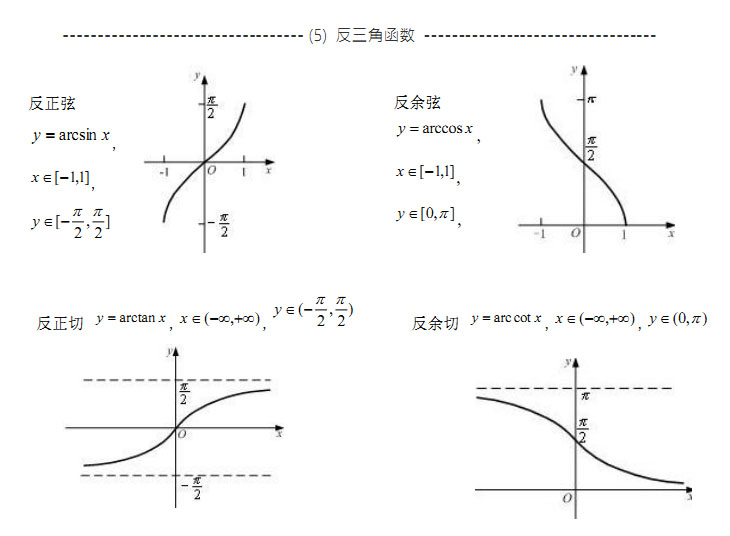
\includegraphics[width=0.9\textwidth,height=0.8\textheight,keepaspectratio]{assets/dec1c90ed6f5c09a1f861de1f18d3e33.png}
\end{center}
\end{frame}

\begin{frame}{单调例题 1：解答}
这些函数本质上都是相应三角函数在其单调区间上的反函数：
\begin{itemize}
  \item $\arcsin x$ 是 $\sin x$ 在 $\left[-\dfrac{\pi}{2},\dfrac{\pi}{2}\right]$ 上的反函数；
  \item $\arccos x$ 是 $\cos x$ 在 $[0,\pi]$ 上的反函数；
  \item $\arctan x$ 是 $\tan x$ 在 $\left(-\dfrac{\pi}{2},\dfrac{\pi}{2}\right)$ 上的反函数；
  \item $\operatorname{arccot}x$ 是 $\cot x$ 在 $(0,\pi)$ 上的反函数。
\end{itemize}
在这些定义区间上，原函数都严格单调且连续，因此由命题 5.5.4，反函数也严格单调且连续。
\end{frame}

\begin{frame}{单调例题 2}
证明：由 Kepler 方程
\[
  y=x-q\sin x,\qquad 0<q<1
\]
可以唯一地确定函数
\[
  x=f(y),
\]
而且它是定义在 $(-\infty,+\infty)$ 上的严格单调增加连续函数。
\end{frame}

\begin{frame}[allowframebreaks]{单调例题 2：解答}
考虑函数
\[
  F(x)=x-q\sin x,\qquad 0<q<1.
\]
显然 $F$ 在 $\R$ 上连续。又因为
\[
  |\sin x|\le 1,
\]
所以当 $x\to\pm\infty$ 时，
\[
  F(x)=x-q\sin x\to\pm\infty,
\]
因此值域为整个 $\R$。
\vspace{0.5em}

再证严格单调性。若 $x_1<x_2$，则
\begin{align*}
  F(x_2)-F(x_1)
  &=(x_2-x_1)-q(\sin x_2-\sin x_1).
\end{align*}
利用不等式
\[
  |\sin x_2-\sin x_1|\le |x_2-x_1|,
\]
可得
\[
  q|\sin x_2-\sin x_1|<|x_2-x_1|.
\]
于是
\[
  F(x_2)-F(x_1)>0.
\]
故 $F$ 严格单调增加。由命题 5.5.4，反函数
\[
  x=f(y)=F^{-1}(y)
\]
定义在 $\R$ 上，并且严格单调增加且连续。
\end{frame}

\begin{frame}
  \centering
  \vspace{1.2cm}
  {\LARGE \bfseries 单调函数练习}
  \vspace{0.8cm}

  {\large 局部单调、稠密集判定、右极限函数与可加单调函数}
\end{frame}

\begin{frame}{单调习题 1}
设函数 $f$ 在开区间 $(a,b)$ 上定义，且对每一点 $x\in(a,b)$，存在邻域 $O(x)$，使得 $f$ 在 $O(x)$ 上单调增加。证明：$f$ 在 $(a,b)$ 上单调增加。
\end{frame}

\begin{frame}[allowframebreaks]{单调习题 1：解答}
任取
\[
  a<c<d<b.
\]
对每个 $x\in[c,d]$，由题设可取邻域 $O(x)$ 使 $f$ 在其上单调增加。由紧性，可从覆盖
\[
  [c,d]\subset \bigcup_{x\in[c,d]} O(x)
\]
中取有限子覆盖。于是存在 $\delta>0$，使得任意
\[
  x,x'\in[c,d],\quad |x-x'|<\delta
\]
时，$x,x'$ 同落在某个覆盖邻域里，从而
\[
  x<x' \Longrightarrow f(x)\le f(x').
\]
将区间 $[c,d]$ 等分为足够细的小段，取分点
\[
  x_k=c+\frac{k}{n}(d-c),\qquad k=0,1,\dots,n,
\]
并使每段长度小于 $\delta$，则
\[
  f(x_0)\le f(x_1)\le \cdots\le f(x_n),
\]
故
\[
  f(c)\le f(d).
\]
由 $c,d$ 任意，$f$ 在 $(a,b)$ 上单调增加。
\end{frame}

\begin{frame}{单调习题 2}
设 $f\in C[a,b]$，且对 $[a,b]$ 内任意两个有理数 $r_1,r_2$，若 $r_1<r_2$，则
\[
  f(r_1)\le f(r_2).
\]
证明：$f$ 在 $[a,b]$ 上单调增加。
\end{frame}

\begin{frame}[allowframebreaks]{单调习题 2：解答}
任取
\[
  a\le x<y\le b.
\]
由有理数稠密性，可取有理数列
\[
  r_n\in\left(x,\frac{x+y}{2}\right),\qquad s_n\in\left(\frac{x+y}{2},y\right),
\]
使
\[
  r_n\to x,\qquad s_n\to y.
\]
并且始终有 $r_n<s_n$，故
\[
  f(r_n)\le f(s_n).
\]
由连续性，
\[
  f(x)=\lim_{n\to\infty}f(r_n)\le \lim_{n\to\infty}f(s_n)=f(y).
\]
因此
\[
  x<y \Longrightarrow f(x)\le f(y),
\]
即 $f$ 在 $[a,b]$ 上单调增加。
\end{frame}

\begin{frame}{单调习题 3}
设 $f$ 是 $(-\infty,+\infty)$ 上的单调函数，在每一点定义
\[
  g(x)=f(x+0).
\]
证明：$g$ 是在 $(-\infty,+\infty)$ 上处处右连续的函数。
\end{frame}

\begin{frame}[allowframebreaks]{单调习题 3：解答}
不妨设 $f$ 单调增加。则
\[
  g(x)=f(x+0)=\inf_{y>x} f(y).
\]
任取 $x\in\R$ 与 $\varepsilon>0$。由下确界定义，存在 $y_1>x$，使
\[
  f(y_1)<\inf_{y>x}f(y)+\varepsilon=g(x)+\varepsilon.
\]
若
\[
  x<x'<y_1,
\]
则由单调性有
\[
  g(x)=\inf_{y>x}f(y)\le g(x')=\inf_{y>x'}f(y)\le f(y_1)<g(x)+\varepsilon.
\]
因此
\[
  |g(x')-g(x)|<\varepsilon,\qquad x<x'<y_1.
\]
这表明
\[
  \lim_{x'\to x+0}g(x')=g(x),
\]
故 $g$ 处处右连续。
\end{frame}

\begin{frame}{单调习题 4}
设 $f$ 为 $(-\infty,+\infty)$ 上的单调函数，且对一切 $x,y\in\R$ 都满足
\[
  f(x+y)=f(x)+f(y).
\]
证明：
\[
  f(x)=f(1)x.
\]
\end{frame}

\begin{frame}[allowframebreaks]{单调习题 4：解答}
先由可加性得
\[
  f(0)=f(0+0)=f(0)+f(0),
\]
故
\[
  f(0)=0.
\]
再由
\[
  0=f(x-x)=f(x)+f(-x),
\]
得
\[
  f(-x)=-f(x).
\]
对正整数 $n$，归纳可得
\[
  f(n)=nf(1).
\]
于是对有理数 $\dfrac{m}{n}$，
\[
  f\!\left(\frac{m}{n}\right)=\frac{m}{n}f(1).
\]
\medskip

这就说明对一切有理数 $r$，都有
\[
  f(r)=rf(1).
\]
\end{frame}

\begin{frame}{单调习题 4：解答（续）}
现任取实数 $x$。取有理数列
\[
  r_n\uparrow x,\qquad s_n\downarrow x.
\]
由单调性，
\[
  f(r_n)\le f(x)\le f(s_n).
\]
而对有理数已知
\[
  f(r_n)=r_n f(1),\qquad f(s_n)=s_n f(1).
\]
令 $n\to\infty$，即得
\[
  xf(1)\le f(x)\le xf(1).
\]
故
\[
  f(x)=f(1)x,\qquad \forall x\in\R.
\]
\end{frame}

\end{document}
